\documentclass[11pt,a4paper]{article}
\usepackage[top=2.54cm,bottom=2.54cm,left=2.6cm,right=2.6cm]{geometry}
\usepackage{setspace}
\onehalfspacing
\setlength{\parindent}{1.2em}
\usepackage{amsmath,amssymb,booktabs,graphicx}
\usepackage[colorlinks=true,linkcolor=black,citecolor=black,urlcolor=blue]{hyperref}
\usepackage{caption}
\captionsetup{font=small,labelfont=bf,skip=6pt}
\graphicspath{{figures/}}

\title{Intestinal metaplasia remains inside the gastritis range of a patient-level epithelial axis}
\author{}
\date{}
\begin{document}
\maketitle

\begin{abstract}
\noindent\textbf{Background.}
Single-cell atlases of gastric mucosa describe epithelial states in gastritis, intestinal metaplasia and gastric cancer. They do not test whether setting one gene to zero moves a patient's epithelial mean from the gastritis pole toward cancer.

\noindent\textbf{Results.}
On GSE249874 (six patients in each group), an epithelial axis was the difference between gastric-cancer and gastritis patient means. Metaplasia was not used to fit the axis. Median projections were 10.26, 11.90 and 18.03. All six metaplasia patients lay inside the gastritis range (9.08--12.51). Cancer (minimum 16.06) did not overlap gastritis (maximum 15.52). Means were 10.98, 11.38 and 17.88. The metaplasia mean had moved 5.8\% of the way from the gastritis mean to the cancer mean. That distance, 6.91, is the axis length, and the largest gene accounts for 4.1\% of it. Of 4{,}781 genes with positive weight and adequate metaplasia detection, 416 passed a pre-specified label shuffle. All 416 also passed every leave-one-out omission. Forty-one further genes passed leave-one-out and stopped at permutation \(p=0.055\). The median retained displacement was 0.0018. The largest, \textit{HSP90AA1}, was 0.24, against a pole gap of 7.77. The nine genes at the smallest attainable \(p\), 0.005, each displaced the metaplasia median by less than 0.005. \textit{CLDN18}, \textit{HNF4G}, \textit{CDX2} and \textit{MUC2} were not retained.

\noindent\textbf{Conclusions.}
In these 18 patients, metaplastic epithelium has not entered the gastric-cancer side of the axis. The axis length is spread across hundreds of genes, and additive single-gene zeroing does not close the gap between gastritis and cancer.
\end{abstract}

\noindent\textbf{Keywords:} gastric cancer; intestinal metaplasia; single-cell RNA sequencing; patient-level projection

\section{Background}

A published 10x atlas profiled 18 gastric specimens, six each of non-atrophic gastritis, intestinal metaplasia and gastric cancer, and recorded \textit{Helicobacter pylori} status \cite{li2025}. That study mapped epithelial, fibroblast and myeloid states along this sequence and nominated \textit{HNF4G} as a transcription-factor candidate for enterocytes inside metaplasia.

Cell-type description and a patient-level shift are different summaries. A marker that is high inside one metaplastic subset need not be the gene that, when set to zero, moves the patient's epithelial mean from gastritis toward cancer. After the epithelial cells of each patient are averaged, the questions are where the three groups sit and how far zeroing one gene moves metaplasia.

The axis and the knockout rule were fixed before the rankings were read. Figure~\ref{fig:position} reports where the 18 patients sit. Figure~\ref{fig:axis} shows how the axis length is divided among genes. Figure~\ref{fig:ko} separates permutation rank from the size of the displacement. The calculation is an additive projection. It is not a dynamical trajectory and not a drug effect.

\section{Methods}

\subsection{Cohort and counts}

The count matrix is GEO series GSE249874 (10x Genomics 3' v3.1, hg38) \cite{li2025}. Eighteen libraries occupy consecutive blocks of 6{,}794{,}880 whitelist barcodes. Barcodes with no counts were discarded (19{,}688{,}657 barcodes had at least one count). Personal names present in GEO titles were not carried into the result tables. The statistical unit is the patient.

Cells were kept when they had at least 200 genes, at least 1{,}000 UMIs, and a ratio of log10(gene count) to log10(UMI count) of at least 0.7. Mitochondrial counts had to be at most 20\%, and haemoglobin-gene counts at most 5\%. These numeric gates are the ones stated in the source paper. DoubletFinder, which that paper also ran, was not repeated. Counts were normalised to 10{,}000 per cell and transformed as \(\log(1+x)\). Gene scores used Scanpy 1.12.3.

\subsection{Epithelial means}

Epithelial score genes were \textit{EPCAM}, \textit{KRT8}, \textit{KRT18} and \textit{KRT19}. Immune score genes were \textit{PTPRC}, \textit{CD3D}, \textit{CD79A} and \textit{MS4A1}. Fibroblast score genes were \textit{COL1A1}, \textit{DCN} and \textit{LUM}. A cell was called epithelial when its epithelial score was positive and higher than both the immune and fibroblast scores. Patients with fewer than 50 epithelial cells would have been dropped; none were. The eleven score genes, mitochondrial genes and haemoglobin genes were excluded from the knockout list. Each patient vector is the mean log expression of that patient's epithelial cells. Patients contribute one vector each. A sample with more epithelial cells does not receive a larger weight.

\subsection{Axis and additive zeroing}

The axis uses the six gastritis and six cancer patients only. The weight of a gene is its mean in cancer minus its mean in gastritis. A gene enters the axis only if it is detected in at least 10\% of epithelial cells in at least four gastritis patients and four cancer patients. A patient's position is the dot product of the patient vector and the weight vector, divided by the Euclidean length of the weight vector. Higher values lie toward cancer. Metaplasia does not enter the fit. Because the weight vector is the difference between the cancer and gastritis means, the difference between those two groups' mean positions equals the length of the weight vector. A gene's share of that length is its squared weight divided by the sum of squared weights.

Zeroing was limited to genes with positive weight that were also detected in at least 10\% of epithelial cells in at least four metaplasia patients. The displacement for a patient is that gene's weight times its value in the patient vector, divided by the same length. The control shuffles the twelve gastritis and cancer labels 200 times (seed 20261003) and leaves metaplasia expression fixed. The permutation \(p\) is \((1+\) the number of null values at least as large as the observed median\()\,/\,201\). That denominator fixes the resolution: \(p\) moves in steps of \(1/201\), and the smallest value the test can return is \(0.005\).

A gene was retained only if that \(p\) was at most 0.05 and if, in at least five of six leave-one-patient omissions, the median of the remaining five metaplasia patients still exceeded the 95th percentile of the null computed on those same five patients. \textit{H. pylori} status was not part of this rule. \textit{CLDN18}, \textit{HNF4G}, \textit{CDX2} and \textit{MUC2} were named in advance and could not change the thresholds.

\section{Results}

\subsection{Cancer separates from gastritis; metaplasia stays inside the gastritis range}

The count and gene gates left 145{,}186 cells. The mitochondrial and haemoglobin gates left 101{,}970. Of these, 19{,}649 were epithelial. Every patient had at least 50 epithelial cells (Table~\ref{tab:patients}).

Epithelial yield was uneven, and it was not balanced across groups (Table~\ref{tab:groups}). The median epithelial count was 2{,}303 in cancer, 812 in gastritis and 466 in metaplasia. Within cancer, GSM7966231 was 51.8\% epithelial (3{,}274 of 6{,}317 cells) and GSM7966226 was 11.2\% (364 of 3{,}262). The lowest yield was metaplasia GSM7966238, 100 epithelial cells out of 7{,}272 (1.4\%). Because each patient enters the axis once, that sample does not dominate the fit, but its mean is estimated from fewer cells.

Summed within groups, epithelial cells were 5{,}030 of 26{,}489 gastritis cells that passed the gates (19.0\%), 2{,}872 of 39{,}018 metaplasia cells (7.4\%) and 11{,}747 of 36{,}463 cancer cells (32.2\%). The median of the six patient-level percentages was 20.2\%, 9.4\% and 33.3\%. The pooled percentage and the median of percentages are different quantities: pooling gives more influence to libraries with more cells, and the axis does not. Within each group, the Spearman coefficient between epithelial-cell count and position was 0.14 in gastritis, $-0.31$ in metaplasia and 0.20 in cancer. Those coefficients were calculated after the positions were known. They were not used to refit the axis.

Median positions were 10.26 in gastritis, 11.90 in metaplasia and 18.03 in cancer (Figure~\ref{fig:position}, Table~\ref{tab:groups}). The means were 10.98, 11.38 and 17.88. The difference between the cancer and gastritis means is 6.91, and that number is the length of the weight vector. The metaplasia mean is 0.40 above the gastritis mean, which is 5.8\% of the way from the gastritis mean to the cancer mean. The lowest cancer patient, GSM7966229, was at 16.06. The highest gastritis patient, GSM7966235, was at 15.52. The poles did not overlap. The six metaplasia patients lay between 9.08 (GSM7966240) and 12.51 (GSM7966239), inside the gastritis minimum (7.87) and maximum (15.52). Their median sits above the gastritis median, but no metaplasia patient has left the gastritis range or entered the cancer range. The nearest metaplasia patient to cancer, GSM7966239, was still 3.55 units below GSM7966229.

\begin{table}[htbp]
  \centering
  \caption{Patients in GSE249874 after the locked cell filters. Each row is one library.}
  \label{tab:patients}
  \footnotesize
  \setlength{\tabcolsep}{4pt}
  \begin{tabular}{llrrrr}
    \toprule
    Patient & \textit{H. pylori} & QC cells & Epithelial cells & Epithelial \% & Position \\
    \midrule
    \multicolumn{6}{l}{\textit{Gastritis}} \\
    GSM7966232 & Negative & 5{,}782 & 508 & 8.8 & 11.77 \\
    GSM7966233 & Negative & 5{,}238 & 1{,}095 & 20.9 & 7.87 \\
    GSM7966234 & Negative & 3{,}290 & 643 & 19.5 & 8.27 \\
    GSM7966235 & Positive & 2{,}481 & 981 & 39.5 & 15.52 \\
    GSM7966236 & Positive & 5{,}471 & 452 & 8.3 & 8.74 \\
    GSM7966237 & Positive & 4{,}227 & 1{,}351 & 32.0 & 13.68 \\
    \addlinespace
    \multicolumn{6}{l}{\textit{Intestinal metaplasia}} \\
    GSM7966238 & Negative & 7{,}272 & 100 & 1.4 & 12.33 \\
    GSM7966239 & Negative & 5{,}538 & 599 & 10.8 & 12.51 \\
    GSM7966240 & Negative & 9{,}225 & 804 & 8.7 & 9.08 \\
    GSM7966241 & Positive & 8{,}153 & 826 & 10.1 & 11.70 \\
    GSM7966242 & Positive & 5{,}840 & 210 & 3.6 & 10.53 \\
    GSM7966243 & Positive & 2{,}990 & 333 & 11.1 & 12.10 \\
    \addlinespace
    \multicolumn{6}{l}{\textit{Gastric cancer}} \\
    GSM7966226 & Negative & 3{,}262 & 364 & 11.2 & 18.94 \\
    GSM7966227 & Negative & 6{,}148 & 536 & 8.7 & 17.11 \\
    GSM7966228 & Negative & 6{,}383 & 2{,}967 & 46.5 & 16.86 \\
    GSM7966229 & Positive & 7{,}962 & 1{,}790 & 22.5 & 16.06 \\
    GSM7966230 & Positive & 6{,}391 & 2{,}816 & 44.1 & 19.30 \\
    GSM7966231 & Positive & 6{,}317 & 3{,}274 & 51.8 & 19.02 \\
    \bottomrule
  \end{tabular}
  \par\vspace{0.35em}
  {\raggedright\footnotesize QC cells are those remaining after the gene, UMI, complexity, mitochondrial and haemoglobin gates. Epithelial \% is epithelial cells divided by QC cells in that patient. Position is the patient's epithelial mean on the gastritis-to-cancer axis. Positions are shown to two decimal places.\par}
\end{table}

\begin{table}[htbp]
  \centering
  \caption{Group summaries. Each group contains six patients, three \textit{H. pylori} positive and three negative.}
  \label{tab:groups}
  \small
  \begin{tabular}{lccc}
    \toprule
     & Gastritis & Metaplasia & Cancer \\
    \midrule
    Position, median & 10.26 & 11.90 & 18.03 \\
    Position, mean & 10.98 & 11.38 & 17.88 \\
    Position, minimum--maximum & 7.87--15.52 & 9.08--12.51 & 16.06--19.30 \\
    Epithelial cells, median & 812 & 466 & 2{,}303 \\
    Epithelial cells, minimum--maximum & 452--1{,}351 & 100--826 & 364--3{,}274 \\
    Epithelial \%, median of patients & 20.2 & 9.4 & 33.3 \\
    \bottomrule
  \end{tabular}
  \par\vspace{0.35em}
  {\raggedright\footnotesize Medians are the average of the third and fourth ordered values. The cancer mean minus the gastritis mean equals the length of the weight vector, 6.91. Epithelial \% is epithelial cells divided by cells remaining after the gates, calculated inside each patient and then summarised across the six patients. The axis was fit with equal weight on the six gastritis and six cancer patients, not with weight proportional to epithelial cell count.\par}
\end{table}

\begin{figure}[htbp]
  \centering
  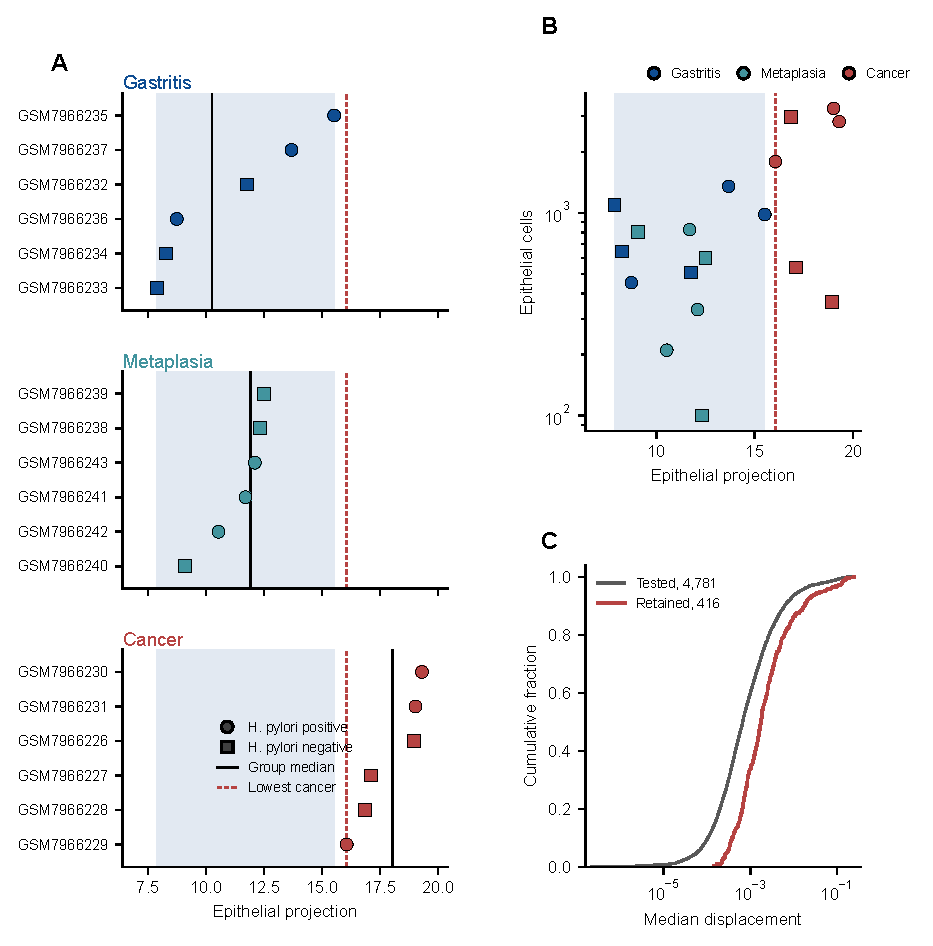
\includegraphics[width=\textwidth]{fig_position.pdf}
  \caption{Patient positions and the size of single-gene displacements. (A)~Each row is one patient, ordered by position within the group. Circles are \textit{H. pylori} positive and squares are negative. The blue band runs from the lowest to the highest gastritis patient. The dashed red line is the lowest cancer patient. The solid black line is that group's median. (B)~Epithelial-cell count against position. The count axis is logarithmic. Colours match panel~A, and marker shape again encodes \textit{H. pylori}. (C)~Cumulative fraction of genes whose median displacement is at or below the value on the horizontal axis. The horizontal axis is logarithmic. Grey is the 4{,}781 tested genes and red is the 416 retained genes. The 7.77-unit gap between gastritis and cancer medians lies to the right of this axis.}
  \label{fig:position}
\end{figure}

\textit{H. pylori} status does not place metaplasia on the cancer side of the axis (Table~\ref{tab:hp}). Each group has three positive and three negative patients. In gastritis the ranges overlap. In metaplasia the positive range lies inside the negative range. In cancer the lowest patient is \textit{H. pylori} positive. This split was not a term in the axis or in the retention rule.

\begin{table}[htbp]
  \centering
  \caption{Position by \textit{H. pylori} status. Entries are the median and the minimum--maximum. Each cell is three patients.}
  \label{tab:hp}
  \small
  \begin{tabular}{lcc}
    \toprule
     & \textit{H. pylori} negative & \textit{H. pylori} positive \\
    \midrule
    Gastritis & 8.27 (7.87--11.77) & 13.68 (8.74--15.52) \\
    Metaplasia & 12.33 (9.08--12.51) & 11.70 (10.53--12.10) \\
    Cancer & 17.11 (16.86--18.94) & 19.02 (16.06--19.30) \\
    \bottomrule
  \end{tabular}
  \par\vspace{0.35em}
  {\raggedright\footnotesize Medians are the middle of the three ordered positions, not a test. The split was not used to fit the axis or to keep genes.\par}
\end{table}

\subsection{No gene carries more than a few percent of the axis}

The median gap of 7.77 is not the length of the axis. The length is the difference between group means, 6.91 (Table~\ref{tab:groups}). Squared weight, divided by the sum of squared weights, is each gene's share of that length (Figure~\ref{fig:axis}). The largest share is 4.1\%, from \textit{PHGR1}, which is higher in gastritis than in cancer. The largest positive share is 3.7\%, from \textit{GAST}. The first four genes together carry 10.3\%. Half of the squared length requires 154 genes, and 90\% requires 1{,}553 of the 7{,}411.

This ranking is not the knockout ranking (Table~\ref{tab:share}). \textit{HSP90AA1} has the largest retained displacement, 0.242, but only 0.8\% of the mean gap. \textit{GAST} has 3.7\% of the mean gap and a metaplasia displacement of 0.0003, because it is barely detected in metaplasia. \textit{FOS} is higher in gastritis, so the retention rule did not test it. Its median displacement is $-0.292$, the largest absolute displacement on the axis, and it is still a few tenths of a unit against a length of 6.91.

\begin{figure}[htbp]
  \centering
  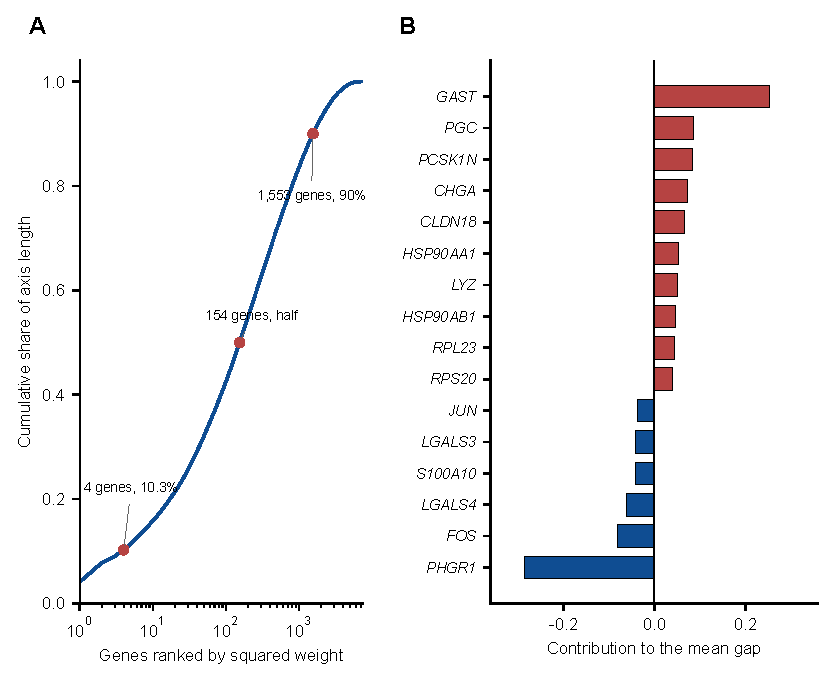
\includegraphics[width=\textwidth]{fig_axis.pdf}
  \caption{How the axis length is divided. (A)~Genes ordered by squared weight. The vertical coordinate is the cumulative share of the squared length, which is also the share of the 6.91-unit gap between group means. The horizontal axis is logarithmic. (B)~Signed contribution of the 16 genes with the largest absolute contributions. Length to the left means the gene is higher in gastritis. The full mean gap is 6.91 and is not drawn on this axis.}
  \label{fig:axis}
\end{figure}

\begin{table}[htbp]
  \centering
  \caption{Largest shares of the mean gap between gastritis and cancer. Ordered by absolute share.}
  \label{tab:share}
  \small
  \begin{tabular}{lrrr}
    \toprule
    Gene & Weight & Share of mean gap (\%) & Displacement \\
    \midrule
    \textit{PHGR1} & $-1.405$ & 4.1 & $-0.084$ \\
    \textit{GAST} & 1.321 & 3.7 & 0.0003 \\
    \textit{PGC} & 0.772 & 1.2 & 0.026 \\
    \textit{PCSK1N} & 0.765 & 1.2 & 0.014 \\
    \textit{FOS} & $-0.745$ & 1.2 & $-0.292$ \\
    \textit{CHGA} & 0.706 & 1.0 & 0.0006 \\
    \textit{CLDN18} & 0.673 & 0.9 & 0.068 \\
    \textit{LGALS4} & $-0.653$ & 0.9 & $-0.134$ \\
    \bottomrule
  \end{tabular}
  \par\vspace{0.35em}
  {\raggedright\footnotesize Share is squared weight divided by the sum of squared weights, expressed as a percentage of the 6.91 mean gap. Displacement is the median change in the six metaplasia positions if that coordinate is set to zero, with the weight vector held fixed. Negative weight was outside the retention rule. Displacements below 0.001 are shown to four decimal places.\par}
\end{table}

\subsection{Genes that pass the null still move the position very little}

The axis contained 7{,}411 genes. Of these, 4{,}781 had positive weight and met the metaplasia detection rule. The retention rule kept 416. Among those 416, the median displacement was 0.0018, the 90th percentile was 0.018, and 21 genes exceeded 0.05. Thirteen exceeded 0.10. The maximum was 0.24 for \textit{HSP90AA1}, which is 3.1\% of the 7.77-unit gap between the gastritis and cancer medians. Fourteen of the 416 genes are ribosomal proteins. \textit{RPS6KC1} is also retained and its symbol begins with \textit{RPS}, but it encodes a kinase and is not one of those fourteen. Three symbols begin with \textit{HSP}: \textit{HSP90AA1}, \textit{HSP90AB1} and \textit{HSPH1}. Figure~\ref{fig:ko} separates permutation rank from displacement for the same 4{,}781 genes. Table~\ref{tab:top} gives the weight, the null 95th percentile and the detection count for the twelve largest retained displacements. All twelve were detected in all six metaplasia patients, and all twelve passed every leave-one-out omission.

\begin{figure}[htbp]
  \centering
  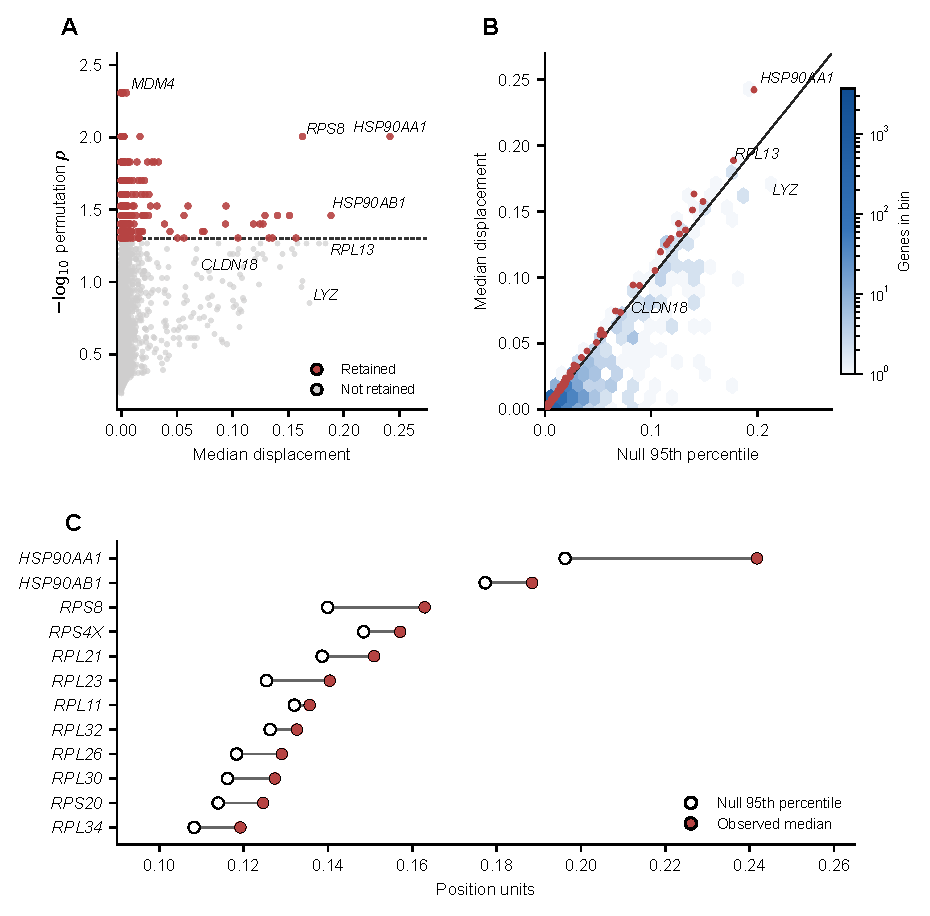
\includegraphics[width=\textwidth]{fig_knockout.pdf}
  \caption{Permutation rank, null percentile and the largest retained displacements. The 4{,}781 points are genes with positive weight detected in at least four metaplasia patients. (A)~Permutation \(p\) against median displacement. The dashed line is \(p=0.05\). Because \(p=(1+k)/201\), points lie on horizontal lines. Red genes were retained. \textit{MDM4} has the largest displacement among the nine genes at \(p=0.005\). \textit{RPL13}, \textit{LYZ} and \textit{CLDN18} are labelled because the displacement is large and the gene was not retained. (B)~Observed displacement against the 95th percentile of the label-shuffle null. Hexagon colour is the gene count in that bin on a logarithmic scale. The diagonal is equality. Red points are the 416 retained genes. (C)~Twelve largest retained displacements. Open circles are the null 95th percentile and filled circles are the observed median. The axis starts at 0.09 so the distance between those two quantities can be read. The 7.77-unit pole gap is not on this axis. No standard-error bars are drawn.}
  \label{fig:ko}
\end{figure}

\begin{table}[htbp]
  \centering
  \caption{Twelve largest retained displacements, with the quantities used by the retention rule.}
  \label{tab:top}
  \footnotesize
  \setlength{\tabcolsep}{3.5pt}
  \begin{tabular}{lrrrrrr}
    \toprule
    Gene & Weight & Displacement & Null 95th & \(p\) & Detected & Leave-one-out \\
    \midrule
    \textit{HSP90AA1} & 0.601 & 0.242 & 0.196 & 0.010 & 6/6 & 6/6 \\
    \textit{HSP90AB1} & 0.562 & 0.188 & 0.177 & 0.035 & 6/6 & 6/6 \\
    \textit{RPS8} & 0.385 & 0.163 & 0.140 & 0.010 & 6/6 & 6/6 \\
    \textit{RPS4X} & 0.444 & 0.157 & 0.148 & 0.050 & 6/6 & 6/6 \\
    \textit{RPL21} & 0.429 & 0.151 & 0.139 & 0.035 & 6/6 & 6/6 \\
    \textit{RPL23} & 0.550 & 0.140 & 0.125 & 0.035 & 6/6 & 6/6 \\
    \textit{RPL11} & 0.320 & 0.136 & 0.132 & 0.050 & 6/6 & 6/6 \\
    \textit{RPL32} & 0.318 & 0.133 & 0.126 & 0.050 & 6/6 & 6/6 \\
    \textit{RPL26} & 0.329 & 0.129 & 0.118 & 0.035 & 6/6 & 6/6 \\
    \textit{RPL30} & 0.291 & 0.127 & 0.116 & 0.040 & 6/6 & 6/6 \\
    \textit{RPS20} & 0.528 & 0.125 & 0.114 & 0.040 & 6/6 & 6/6 \\
    \textit{RPL34} & 0.333 & 0.119 & 0.108 & 0.040 & 6/6 & 6/6 \\
    \bottomrule
  \end{tabular}
  \par\vspace{0.35em}
  {\raggedright\footnotesize Weight is the cancer mean minus the gastritis mean on the log scale. Displacement is the median, over six metaplasia patients, of weight times that patient's expression, divided by the length of the weight vector. Null 95th is the 95th percentile of the same median under 200 label shuffles. \(p=(1+\)number of null medians at least as large as observed\()\,/\,201\). Detected counts metaplasia patients in whom at least 10\% of epithelial cells express the gene. Leave-one-out counts how many of the six five-patient medians still exceeded their own null 95th percentile.\par}
\end{table}

\subsection{Permutation rank is not the size of the displacement}

The tested set is a subset of the axis (Table~\ref{tab:filter}). Of 7{,}411 axis genes, 2{,}261 had negative weight. Setting one of those genes to zero would raise the projection, so they were outside the locked contrast, which keeps only positive weights. Of the 5{,}150 genes with positive weight, 369 were detected in fewer than four metaplasia patients and were not tested. The remaining 4{,}781 were tested. Every gene that passed \(p\le 0.05\) also passed all six leave-one-out omissions, so that second rule removed nobody from this matrix. The 416 retained genes are the tested genes with \(p\le 0.05\).

Forty-one tested genes passed at least five leave-one-out omissions and had \(p=0.055\), which is \(11/201\), one null count past the locked threshold. All 41 share that same \(p\). The threshold was not moved after the count was seen. Four of the 41 displaced the metaplasia median by more than 0.10 (Table~\ref{tab:boundary}). \textit{RPL13}, the largest, moved it by 0.184 against a null 95th percentile of 0.177. \textit{LYZ} was not in that set: its displacement was 0.169, its null 95th percentile was 0.211, and its leave-one-out count was 0/6.

Nine tested genes reached \(p=0.005\), the smallest value this permutation returns. Their displacements ran from 0.0002 (\textit{LDLRAP1}) to 0.0048 (\textit{MDM4}). All nine were retained. None of them is among the twelve largest displacements, so a sort by \(p\) does not recover Table~\ref{tab:top}.

Weight was a different ranking again (Table~\ref{tab:weight}). The five largest positive weights were not retained. \textit{GAST} had weight 1.321 and was detected in one of six metaplasia patients, so it was not tested; its displacement was 0.0003. \textit{HSP90AA1}, weight 0.601, was the sixth-largest positive weight and the largest that was retained.

Of the 416 retained displacements, 359 were below 0.01. For 406 of the 416, the displacement exceeded its own null 95th percentile by less than 0.01. The median of that excess was 0.0002.

\begin{table}[htbp]
  \centering
  \caption{Genes at each locked rule. Counts are from the axis table, not a second fit.}
  \label{tab:filter}
  \small
  \begin{tabular}{p{0.78\textwidth}r}
    \toprule
    Rule & Genes \\
    \midrule
    On the axis & 7{,}411 \\
    Negative weight & 2{,}261 \\
    Positive weight & 5{,}150 \\
    Positive weight, detected in fewer than four metaplasia patients & 369 \\
    Tested & 4{,}781 \\
    Leave-one-out passed and permutation \(p>0.05\) & 41 \\
    Retained & 416 \\
    Retained, displacement \(<0.01\) & 359 \\
    Retained, excess over the null 95th percentile \(<0.01\) & 406 \\
    Retained, leave-one-out 6/6 & 416 \\
    \bottomrule
  \end{tabular}
  \par\vspace{0.35em}
  {\raggedright\footnotesize Tested means positive weight and detection in at least 10\% of epithelial cells in at least four metaplasia patients. Leave-one-out passed means the five-patient median beat its own null 95th percentile in at least five of six omissions. Excess is the observed median displacement minus that gene's null 95th percentile. Every retained gene passed all six omissions, so the leave-one-out rule did not remove any gene that had already passed \(p\le 0.05\).\par}
\end{table}

\begin{table}[htbp]
  \centering
  \caption{Tested genes with displacement above 0.10 that stopped at \(p=0.055\). Column definitions match Table~\ref{tab:top}.}
  \label{tab:boundary}
  \footnotesize
  \setlength{\tabcolsep}{3.5pt}
  \begin{tabular}{lrrrrrr}
    \toprule
    Gene & Weight & Displacement & Null 95th & \(p\) & Detected & Leave-one-out \\
    \midrule
    \textit{RPL13} & 0.357 & 0.184 & 0.177 & 0.055 & 6/6 & 6/6 \\
    \textit{RPL13A} & 0.453 & 0.178 & 0.174 & 0.055 & 6/6 & 6/6 \\
    \textit{RPS11} & 0.468 & 0.166 & 0.161 & 0.055 & 6/6 & 6/6 \\
    \textit{RPL12} & 0.291 & 0.125 & 0.116 & 0.055 & 6/6 & 6/6 \\
    \bottomrule
  \end{tabular}
  \par\vspace{0.35em}
  {\raggedright\footnotesize These four are the members of the 41-gene boundary set with displacement above 0.10. All 41 have \(p=11/201=0.055\). None was retained. The cutoff was not changed to include them.\par}
\end{table}

\begin{table}[htbp]
  \centering
  \caption{Largest positive weights that were not retained.}
  \label{tab:weight}
  \footnotesize
  \setlength{\tabcolsep}{3.5pt}
  \begin{tabular}{lrrrrr}
    \toprule
    Gene & Weight & Displacement & Detected & \(p\) & Leave-one-out \\
    \midrule
    \textit{GAST} & 1.321 & 0.0003 & 1/6 & --- & --- \\
    \textit{PGC} & 0.772 & 0.026 & 5/6 & 0.204 & 0/6 \\
    \textit{PCSK1N} & 0.765 & 0.014 & 3/6 & --- & --- \\
    \textit{CHGA} & 0.706 & 0.0006 & 1/6 & --- & --- \\
    \textit{CLDN18} & 0.673 & 0.068 & 5/6 & 0.090 & 0/6 \\
    \textit{LYZ} & 0.593 & 0.169 & 6/6 & 0.139 & 0/6 \\
    \bottomrule
  \end{tabular}
  \par\vspace{0.35em}
  {\raggedright\footnotesize A dash means the gene was not tested: detection in metaplasia was below four patients. \textit{CLDN18} is repeated from Table~\ref{tab:pre} because it is the fifth-largest positive weight. \textit{HSP90AA1} (weight 0.601) is the next positive weight and was retained. Displacements below 0.001 are shown to four decimal places.\par}
\end{table}

\subsection{Pre-specified genes are not retained}

None of the four genes named before the ranking was retained (Table~\ref{tab:pre}). \textit{CLDN18} had a positive weight and a displacement of 0.068, with permutation \(p=0.090\) and no leave-one-out pass. \textit{HNF4G} had a negative weight, so it is higher on the gastritis side of this axis; its displacement was \(-0.002\). \textit{CDX2} and \textit{MUC2} never entered the axis, because they were not detected at the 10\% threshold in at least four gastritis patients and four cancer patients. That filter does not measure whether either gene is expressed inside metaplasia alone.

\begin{table}[htbp]
  \centering
  \caption{Genes named before the ranking was inspected. Column definitions match Table~\ref{tab:top}.}
  \label{tab:pre}
  \small
  \begin{tabular}{lrrrrl}
    \toprule
    Gene & Weight & Displacement & \(p\) & Leave-one-out & Decision \\
    \midrule
    \textit{CLDN18} & 0.673 & 0.068 & 0.090 & 0/6 & Not retained \\
    \textit{HNF4G} & $-0.142$ & $-0.002$ & 0.985 & 0/6 & Not retained \\
    \textit{CDX2} & --- & --- & --- & --- & Not on the axis \\
    \textit{MUC2} & --- & --- & --- & --- & Not on the axis \\
    \bottomrule
  \end{tabular}
  \par\vspace{0.35em}
  {\raggedright\footnotesize A dash means the gene failed the axis filter: detection in at least 10\% of epithelial cells in at least four gastritis patients and four cancer patients. \textit{HNF4G} has a negative weight, so zeroing it does not move metaplasia toward gastritis.\par}
\end{table}

For 415 of the 416 retained genes, the displacement was positive in all three \textit{H. pylori}-positive metaplasia patients and all three negative ones. The exception was \textit{ONECUT3} (median displacement 0.0019, permutation \(p=0.040\)), positive in three positive patients and two negative patients. This count was not a test of \textit{H. pylori}, and it was not used to keep or drop genes.

\section{Discussion}

The two poles of this axis separate: every cancer patient sits above every gastritis patient. Metaplasia does not occupy the interval between those clouds. Its median is between the two group medians, and that fact is easy to over-read. All six metaplasia patients remain inside the gastritis range. On the means, the over-reading is sharper. The metaplasia mean is 0.40 above the gastritis mean, 5.8\% of the 6.91-unit axis length, and the nearest metaplasia patient is still 3.55 units below the lowest cancer patient.

The length itself is not a single coordinate (Figure~\ref{fig:axis}). Four genes carry 10.3\% of it, 154 carry half, and the largest share is 4.1\%. \textit{HSP90AA1} can head the knockout list and still be only 0.8\% of that length, because a displacement depends on how strongly metaplasia expresses the gene, not only on the gene's weight. \textit{FOS} shows the same split from the other side: its displacement is the largest absolute value on the axis, $-0.292$, and its share of the length is 1.2\%. Neither ranking produces a gene that accounts for the poles.

The 416 retained genes clear a null that is itself narrow. Clearing it is not evidence that a single gene accounts for the pole gap. Only 13 of them move the metaplasia median by more than 0.10, and the largest displacement is 3.1\% of the 7.77-unit gap. For 406 of the 416, the excess over the gene's own null 95th percentile is below 0.01. The genes at the top of Table~\ref{tab:top} are heat-shock and ribosomal genes whose epithelial means are higher in cancer than in gastritis. They are not, on this calculation, nodes whose removal repositions a metaplasia patient onto the cancer side. The same table also shows that several of these genes sit close to their own null: \textit{RPL11} has displacement 0.136 against a null 95th percentile of 0.132. A pass at \(p=0.050\) is the edge of a 200-shuffle resolution, not a large effect.

The boundary one count past that edge is the same kind of result. \textit{RPL13}, \textit{RPL13A}, \textit{RPS11} and \textit{RPL12} cleared every leave-one-out omission and stopped at \(p=0.055\). Their displacements are the same order as the genes that were retained, and they remain far below the pole gap. Including them would be a different rule from the one locked before the ranking.

The largest weights are a third ranking, and it does not recover a shift of metaplasia either. \textit{GAST} and \textit{CHGA} are high on the cancer side of the axis and barely detected in metaplasia, so setting them to zero changes the metaplasia position by less than 0.001. \textit{PGC} is detected in five of six metaplasia patients and still fails the null. The nine genes with the smallest permutation \(p\) are retained and almost stationary: \textit{MDM4}, the largest of them, moves the median by 0.0048. Sorting the tested set by \(p\) and sorting it by displacement answer different questions.

\textit{HNF4G} was nominated in the source atlas as a transcription-factor candidate for enterocytes within metaplasia \cite{li2025}. On the patient axis fit here, its weight is negative and it fails retention. The two statements use different aggregations. One describes a cell subset inside metaplasia. The other describes the difference between gastritis and cancer patient means. Failure of \textit{CDX2} and \textit{MUC2} to enter the axis likewise does not show that they are absent from metaplastic epithelium.

\subsection{Limitations}

Each group has six patients, and one metaplasia sample contributes only 100 epithelial cells, so that patient's mean is less stable than the others. The axis was not refit after removing one gastritis or one cancer patient, so the shares in Table~\ref{tab:share} describe the locked fit only. \textit{H. pylori} status, balanced as three positive and three negative patients per group, was not a term in the primary test. Zeroing one coordinate leaves every other gene unchanged, so the displacement ignores compensation. The source paper's doublet filter was not repeated. These boundaries belong to the claims above: the separation of the poles, the location of metaplasia, and the size of single-gene displacements are descriptions of this matrix under the locked rule, not a treatment ranking.

\section{Conclusions}

On GSE249874, a patient-level epithelial projection separates six gastric cancers from six gastritis samples. Six intestinal-metaplasia samples remain inside the gastritis range, and the metaplasia mean has moved 5.8\% of the 6.91-unit axis length. No gene accounts for more than 4.1\% of that length. Under the pre-specified rule, 416 genes are retained, and none of their displacements approaches the gap between the groups. \textit{CLDN18}, \textit{HNF4G}, \textit{CDX2} and \textit{MUC2} are not retained.

\section*{Declarations}

\subsection*{Ethics approval and consent to participate}
This study reanalysed the public series GSE249874. No new human specimens were collected.

\subsection*{Consent for publication}
Not applicable.

\subsection*{Competing interests}
To be completed by the authors.

\subsection*{Funding}
To be completed by the authors.

\subsection*{Authors' contributions}
To be completed by the authors.

\subsection*{Data availability}
The count matrix is available from GEO under accession GSE249874. Patient positions and gene-level displacements calculated for this paper are stored with the analysis record. The analysis script has not been deposited in a public code archive.

\subsection*{Abbreviations}
GEO: Gene Expression Omnibus; UMI: unique molecular identifier.

\begin{thebibliography}{9}
\bibitem{li2025}
Li N, Chen S, Xu X, Wang H, Zheng P, Fei X, et al.
Single-cell transcriptomic profiling uncovers cellular complexity and microenvironment in gastric tumorigenesis associated with \textit{Helicobacter pylori}.
J Adv Res. 2025;74:471--491.
doi:10.1016/j.jare.2024.10.012.
\end{thebibliography}

\end{document}
